% !TeX root = er.tex

\chapter{Comportamento Reativo}\label{ch.reactive}

Estamos agora prontos para escrever nossos primeiros algoritmos para robôs. Estes algoritmos demonstram o \emph{comportamento reativo}: um evento (como a detecção de um objeto próximo pelo robô) faz com que o robô reaja realizando uma ação que altera seu comportamento (como a parada dos motores). Comportamento puramente reativo ocorre quando a ação está relacionada apenas à ocorrência de um evento e não depende de dados armazenados na memória (estado).

Os comportamentos reativos são aqueles dos veículos chamados \emph{Braitenberg}, que são apropriados para introduzir a robótica porque comportamentos complexos surgem a partir de algoritmos simples. As seções~\ref{s.braitenberg}--\ref{s.turning} descrevem veículos Braitenberg que demonstram comportamento reativo; no capítulo~\ref{ch.fmg} apresentamos veículos Braitenberg que têm comportamento não reativo com estados. A seção~\ref{s.line} apresenta vários algoritmos para o comportamento reativo clássico dos seguidores de linha. O seguimento de linha é uma tarefa interessante porque os algoritmos são sensíveis às características dos sensores e das linhas. Calibração é necessária para determinar os limites ideais para o movimento rápido e robusto do robô. A seção~\ref{s.abstract-vehicles} dá uma breve visão geral da formulação original dos veículos de Braitenberg em uma abordagem biológica com sensores conectados diretamente aos motores, e não através de um computador. Mais tarde no livro (Sect.~\ref{s.braitenberg-ann}) discutimos a implementação de veículos Braitenberg usando redes neurais.

\section{Veículos Braitenberg}\label{s.braitenberg}

Valentino Braitenberg foi um neurocientista que descreveu o projeto de veículos virtuais que apresentavam um comportamento surpreendentemente complexo. Os pesquisadores do MIT Media Lab desenvolveram implementações de hardware dos veículos a partir de \emph{tijolos programáveis}, que foram os precursores dos kits de robótica Mindstorms, da \lego.\footnote{O relatório do MIT usa o termo "criaturas Braitenberg", mas mantemos o termo original.} Este capítulo descreve uma implementação da maioria dos veículos Braitenberg a partir do relatório do MIT. O hardware do MIT usou sensores de luz e de toque, enquanto nosso robô genérico se baseia em sensores de proximidade horizontais.

Para facilitar a comparação com o relatório MIT (e, indiretamente, com o livro do Braitenberg), os nomes de seus veículos foram mantidos, embora possa ser difícil entender seu significado em nossas implementações.

Dois veículos são apresentados em detalhes com o seguinte:
\begin{itemize}
\item A especificação do comportamento do robô;
\item Um algoritmo formalizado para o comportamento especificado;
\item Uma atividade que lhe pede para implementar o algoritmo em seu robô.
\end{itemize}
Os outros veículos são apresentados em atividades que especificam o comportamento e lhe pedem para desenvolver um algoritmo e implementá-lo em seu robô.

\section{Reagindo à Detecção de um Objeto}\label{s.reacting}

\begin{quote}
\normalsize\noindent{}\textbf{Especificação (Tímido):} Quando o robô não detecta um objeto, ele se move para a frente. Quando ele detecta um objeto, ele pára.
\end{quote}
\noindent{}O algoritmo~\ref{alg.timid} implementa este comportamento.

\begin{figure}
\begin{alg}{Tímido}{timid}
\hline
\stl{}&when object not detected in front&// Quando objeto não é detectado em frente\\
\stl{}&\idc{} left-motor-power \ass $100$&\\
\stl{}&\idc{} right-motor-power \ass $100$&\\
\stl{}&&\\
\stl{}&when object detected in front&// Quando objeto é detectado em frente\\
\stl{}&\idc{} left-motor-power \ass $0$&\\
\stl{}&\idc{} right-motor-power \ass $0$&\\
\end{alg}
\end{figure}

O algoritmo utiliza dois gerenciadores de eventos, um para o evento de detecção de um objeto e outro para o evento de não detecção de um objeto. Os gerenciadores de eventos são escritos usando a declaração \p{when} cujo significado é:

\begin{center}
\p{Quando (when) o evento \emph{ocorre pela primeira vez}, execute as seguintes ações}.
\end{center}
\noindent{}Por que usamos esta construção e não a declaração mais familiar \p{while} (Algoritmo~\ref{alg.timid-a})?

\begin{figure}
\begin{alg}{Tímido com while}{timid-a}
\hline
\stl{}&while object not detected in front&// Quando objeto não é detectado em frente\\
\stl{}&\idc{} left-motor-power \ass $100$&\\
\stl{}&\idc{} right-motor-power \ass $100$&\\
\stl{}&&\\
\stl{}&while object detected in front&// Quando objeto é detectado em frente\\
\stl{}&\idc{} left-motor-power \ass $0$&\\
\stl{}&\idc{} right-motor-power \ass $0$&\\
\end{alg}
\end{figure}

Se usarmos a declaração de \p{while}, enfatizaremos que \emph{enquanto} o objeto não for detectado, os motores serão ligados e \emph{enquanto} o objeto for detectado, os motores serão desligados. Como o sensor detectará o objeto em uma faixa de distâncias, os motores serão ligados ou desligados repetidamente. É provável que nenhum dano será feito se um motor já desligado for desligado e um motor já ligado for ligado, mas estes comandos repetidos não são necessários e podem desperdiçar recursos. Portanto, preferimos desligar os motores somente quando o objeto for detectado pela primeira vez e ligá-los somente quando o objeto não for detectado pela primeira vez. A declaração \p{when} dá a significado ao que queremos fazer.

\begin{framed}
\act{Tímido}{timid}
\begin{itemize}
\item Implemente o comportamento Tímido.
\end{itemize}
\end{framed}

\begin{framed}
\act{Indeciso}{indecisive}
\begin{itemize}
\item Implemente o comportamento indeciso.
\begin{quote}
\normalsize\noindent\textbf{Especificação (Indeciso):} Quando o robô não detecta um objeto, ele se move para a frente. Quando detecta um objeto, ele se move para trás.
\end{quote}
\item Na distância certa, o robô irá se mover para frente e para trás em rápida sucessão. Meça esta distância para seu robô e para objetos de reflexividade diferente.
\end{itemize}
\end{framed}

\begin{framed}
\act{Obstinado}{dogged}
\begin{itemize}
\item Implemente o comportamento Obstinado.
\begin{quote}
\normalsize\noindent\textbf{Especificação (Obstinado):} Quando o robô detecta um objeto na frente, ele se move para trás. Quando o robô detecta um objeto atrás, ele se move para frente.
\end{quote}
\end{itemize}
\end{framed}

\begin{framed}
\act{Obstinado (parar)}{dogged1}
\begin{itemize}
\item Implemente o comportamento Obstinado (parar).
\begin{quote}
\normalsize\noindent\textbf{Especificação (Obstinado (parar)):} Como em Activity~\ref{act.dogged}, mas quando um objeto não é detectado, o robô pára.
\end{quote}
\end{itemize}
\end{framed}

\begin{framed}
\act{Atraente e repulsivo}{attractive}
\begin{itemize}
\item Implemente o comportamento atraente e repulsivo.
\begin{quote}
\normalsize\noindent\textbf{Especificação (Atraente e repulsivo):} Quando um objeto se aproxima do robô por trás, o robô foge até ficar fora de alcance.
\end{quote}
\end{itemize}
\end{framed}

\section{Reagindo e virando}\label{s.turning}

Um carro gira mudando o ângulo de suas rodas dianteiras em relação à estrutura do veículo. A potência do motor não é alterada. Um robô com tração diferencial não tem mecanismo de direção (como o volante de um carro ou o guidão de uma bicicleta). Ao invés disso, ele gira ajustando diferentes velocidades para as rodas esquerda e direita. Se uma roda gira mais rápido do que a outra, o robô gira na direção oposta à da roda mais rápida (Fig.~\ref{fig.left-gentle}). Se uma roda gira para trás enquanto a outra gira para frente, a curva é muito mais fechada (Fig.~\ref{fig.left-sharp}). Nas figuras, as setas denotam a direção e velocidade de cada roda. O emph{raio de giro} é o raio do círculo que é o caminho do robô. Dizemos que uma curva é mais fechada se o raio for menor. No extremo, se uma roda gira para frente e a segunda gira para trás à mesma velocidade, o robô gira em torno de seu próprio eixo e o raio de giro é zero.

\begin{figure}
\begin{minipage}{.45\textwidth}
\begin{tikzpicture}
\pic[rotate=10,scale=1.2] at (0,0) { robot };
\draw[raxis] (0,0mm) -- (-80:15mm);
\draw[raxis] (0,0mm) -- (100:15mm);
\draw[raxis] (0,0) -- (10:8pt);
\draw[raxis] (0,0) -- (190:8pt);
\draw[->] (6mm,-8.5mm) -- +(10:15mm);
\draw[->] (3mm,10.3mm) -- +(10:5mm);
\end{tikzpicture}
\caption{Curva suave à esquerda}\label{fig.left-gentle}
\end{minipage}
\hspace{\fill}
\begin{minipage}{.45\textwidth}
\begin{tikzpicture}
\pic[rotate=45,scale=1.2] at (0,0) { robot };
\draw[raxis] (0,0mm) -- (-45:15mm);
\draw[raxis] (0,0mm) -- (135:15mm);
\draw[raxis] (0,0) -- (45:8pt);
\draw[raxis] (0,0) -- (225:8pt);
\draw[->] (9.6mm,-3.6mm) -- +(45:15mm);
\draw[->] (-9.5mm,3.7mm) -- +(-135:5mm);
\end{tikzpicture}
\caption{Curva fecahda à esquerda}\label{fig.left-sharp}
\end{minipage}
\end{figure}
%
%\begin{figure}
%\subfigures
%\begin{minipage}{\textwidth}
%\leftfigure[c]{
%\begin{tikzpicture}
%\pic[rotate=10,scale=1.2] at (0,0) { robot };
%\draw[raxis] (0,0mm) -- (-80:15mm);
%\draw[raxis] (0,0mm) -- (100:15mm);
%\draw[raxis] (0,0) -- (10:8pt);
%\draw[raxis] (0,0) -- (190:8pt);
%\draw[->] (6mm,-8.5mm) -- +(10:15mm);
%\draw[->] (3mm,10.3mm) -- +(10:5mm);
%\end{tikzpicture}
%}
%\hspace{\fill}
%\rightfigure[c]{
%\begin{tikzpicture}
%\pic[rotate=45,scale=1.2] at (0,0) { robot };
%\draw[raxis] (0,0mm) -- (-45:15mm);
%\draw[raxis] (0,0mm) -- (135:15mm);
%\draw[raxis] (0,0) -- (45:8pt);
%\draw[raxis] (0,0) -- (225:8pt);
%\draw[->] (9.6mm,-3.6mm) -- +(45:15mm);
%\draw[->] (-9.5mm,3.7mm) -- +(-135:5mm);
%\end{tikzpicture}
%}
%\leftcaption{Gentle left turn\label{fig.left-gentle}}
%\rightcaption{Sharp left turn\label{fig.left-sharp}}
%\end{minipage}
%\end{figure}

Vamos agora implementar um veículo Braitenberg cuja especificação requer que o robô gire.

\begin{quote}
\normalsize\noindent\textbf{Especificação (Paranóico):} Quando o robô detecta um objeto, ele se move para a frente (colidindo com o objeto). Quando não detecta um objeto, ele se gira para a esquerda.
\end{quote}
Algoritmo~\ref{alg.paranoid} implementa esse comportamento.

\smallskip

\begin{alg}{Paranóico}{paranoid}
\hline
\stl{}&when object detected in front&// Quando um objeto é\\
&&//\idc{}detectado à frente\\
\stl{}&\idc{} left-motor-power \ass $100$&\\
\stl{}&\idc{} right-motor-power \ass $100$&\\
\stl{}&&\\
\stl{}&when object not detected in front&// Quando nenhum objeto\\
&&// \idc{}é detectado à frente\\
\stl{}&\idc{} left-motor-power \ass $-50$&// Motor esquerdo gira para trás\\
\stl{}&\idc{} right-motor-power \ass $50$&// Motor direito gira para frente\\
\end{alg}

\begin{framed}
\act{Paranóico}{paranoid}
\begin{itemize}
\item Implemente o comportamento paranóico.
\item No algoritmo, os motores esquerdo e direito são definidos para potências iguais, mas opostas. Experimente com estes níveis de potência para ver sua influência no raio de giro do robô.
\end{itemize}
\end{framed}

\begin{framed}
\act{Paranóico (direita-esquerda)}{paranoid1}
\begin{itemize}
\item Implemente o comportamento paranóico (direita-esquerda).
\begin{quote}
\normalsize\noindent\textbf{Especificação (Paranóico (direita-esquerda)):}
Quando um objeto é detectado na frente do robô, o robô se move para a frente. Quando um objeto é detectado à direita do robô, o robô vira à direita. Quando um objeto é detectado à esquerda do robô, o robô vira à esquerda. Quando nenhum objeto é detectado, o robô não se move.
\end{quote}
\end{itemize}
\end{framed}

\begin{framed}
\act{Inseguro}{insecure}
\begin{itemize}
\item Implemente o comportamento inseguro.
\begin{quote}
\normalsize\noindent\textbf{Especificação (Inseguro):} Se um objeto não for detectado à esquerda do robô, defina o motor direito para girar para frente e o motor esquerdo para não girar. Se um objeto for detectado à esquerda do robô, desative o motor direito e defina o motor esquerdo para girar para a frente.
\end{quote}
\item Experimente os ajustes do motor até que o robô siga uma parede à sua esquerda.
\end{itemize}
\end{framed}

\begin{framed}
\act{Dedicado}{driven}
\begin{itemize}
\item Implemente o comportamento Dedicado.
\begin{quote}
\normalsize\noindent\textbf{Especificação (Dedicado):} Se um objeto for detectado à esquerda do robô, defina o motor direito para girar para frente e o motor esquerdo para não girar. Se um objeto for detectado à direita do robô, desative o motor direito e defina o motor esquerdo para girar para frente.
\end{quote}
\item Experimentar os ajustes do motor até o robô se aproximar do objeto em ziguezague.
\end{itemize}
\end{framed}

\section{Seguimento de Linha}\label{s.line}

Considere um armazém com carrinhos robóticos que tragam objetos para uma área central de despacho (Fig.~\ref{fig.warehouse}). Linhas são pintadas no piso do armazém e o robô é instruído a segui-las até chegar ao depósito do objeto desejado.

\begin{figure}
\begin{center}
\begin{tikzpicture}[thick, rounded corners, shelf/.style={draw, minimum height=1.2cm, rectangle split, rectangle split parts=2}]
\draw  (-.8,2.0) -- (-.8,1.7) -- (2.2,1.7) -- (2.2,0) -- (3.6,0) -- (3.6,1.7) -- (5.0,1.7) -- (5.0,0) -- (6.6,0) -- (6.6,2.8) -- (-.8,2.8) -- (-.8,2.6);
\node[draw, shape=rectangle, minimum height=1pt] at (-.8,2.3) {\textsf{Despacho}};
\node[shelf] at (1.5,.8) {\textsf{A}\nodepart{two}\textsf{B}};
\node[shelf] at (2.9,.8) {\textsf{C}\nodepart{two}\textsf{D}};
\node[shelf] at (4.3,.8) {\textsf{E}\nodepart{two}\textsf{F}};
\node[shelf] at (5.7,.8) {\textsf{G}\nodepart{two}\textsf{H}};
\end{tikzpicture}
\caption{Um armazém robótico}\label{fig.warehouse}
\end{center}
\end{figure}

\emph{Seguimento de linha} é uma tarefa que traz à tona toda a incerteza da construção de robôs no mundo real. A linha pode não ser perfeitamente reta, sujeira pode obscurecer parte da linha, ou poeira pode fazer com que uma roda se mova mais lentamente do que a outra. Para seguir uma linha, o robô deve decidir se está na linha ou não e, se começar a sair da linha, deve virar na direção correta para retornar a ela.

\subsection{Seguimento de linha com um par de sensores de solo}

Para seguir uma linha, um par de sensores de solo pode ser utilizado (Fig.~\ref{fig.ground-on-a-line}).\footnote{A figura mostra uma vista de cima, embora os sensores de solo estejam na parte inferior do robô.} Um sensor de solo em um piso de cor clara detectará muita luz refletida. Se uma linha escura for pintada no chão, o sensor detectará muito pouca luz refletida quando estiver sobre a linha.\footnote{Se seu piso for de cor escura, uma linha branca deve ser usada.} A linha deve ser preta para maior contraste com o piso branco, mas a figura exibe a linha em cinza claro para não obscurecer o robô e seus sensores. Limiares são usados para determinar quando ocorre o evento de um sensor passando da detecção da linha para a detecção do chão ou vice-versa.

\begin{figure}
\begin{center}
\begin{tikzpicture}[scale=1.1]
\draw[fill,lightgray] (-2,-3.5mm) rectangle +(7,8mm);
\pic at (0,0) { robot2 };
\end{tikzpicture}
\caption{Um robô com dois sensores de solo sobre uma linha}\label{fig.ground-on-a-line}
\end{center}
\end{figure}

A linha deve ser suficientemente larga para que ambos os sensores de solo a detectem quando o robô estiver diretamente acima dela. Os sensores não precisam estar totalmente sobre a linha; é suficiente que a quantidade de luz refletida da linha para o sensor esteja abaixo do limiar definido.

Para implementar o seguimento da linha, o robô deve avançar sempre que ambos os sensores detectarem uma superfície escura, indicando que ele está na linha. Se o robô começar a sair da linha, um dos sensores de solo esquerdo ou direito deixará a linha primeiro (Fig.~\ref{fig.leave-left-right}):

\begin{figure}
\begin{center}
\begin{tikzpicture}[scale=1.1]
\draw[fill,lightgray] (-1,-3.5mm) rectangle +(7,8mm);
\pic[rotate=10] at (0,3mm) { robot2 };
\pic[rotate=-10] at (4,-3mm) { robot2 };
\end{tikzpicture}
\caption{Deixando a linha\label{fig.leave-left-right}}
\end{center}
\end{figure}

\begin{itemize}
\item Se o robô sair da linha para a \emph{esquerda}, o sensor da \emph{esquerda} não detectará a linha enquanto o sensor da \emph{direita} ainda a estiver detectando; o robô deve virar para a \emph{direita}.
\item Se o robô sair da linha para a \emph{direita}, o sensor da \emph{direita} não detectará a linha enquanto o sensor da esquerda ainda a estiver detectando; o robô deve virar para a \emph{esquerda}.
\end{itemize}
Por enquanto, especificamos que o robô pára sempre que nenhum dos sensores detecta a linha.

O algoritmo~\ref{alg.line-two} formaliza a descrição apresentada anteriormente.

\begin{figure}
\begin{alg}{Seguimento de linha com dois sensores}{line-two}
\hline
\stl{}&when both sensors detect black&// Quando ambos sensores\\
&&//\idc{}detectam preto (linha)\\
\stl{}&\idc{} left-motor-power \ass $100$&\\
\stl{}&\idc{} right-motor-power \ass $100$&\\
\stl{}&&\\
\stl{}&when neither sensor detects black&// Quando nenhum sensor\\
&&//\idc{}detecta preto\\
\stl{}&\idc{} left-motor-power \ass $0$&\\
\stl{}&\idc{} right-motor-power \ass $0$&\\
\stl{}&&\\
\stl{}&when only the left sensor detects black&// Quando apenas o sensor\\
&&//\idc{}esquerdo detecta preto\\
\stl{}&\idc{} left-motor-power \ass $0$&\\
\stl{}&\idc{} right-motor-power \ass $50$&\\
\stl{}&&\\
\stl{}&when only the right sensor detects black&// Quando apenas o sensor\\
&&//\idc{}direito detecta preto\\
\stl{}&\idc{} left-motor-power \ass $50$&\\
\stl{}&\idc{} right-motor-power \ass $0$&\\
\end{alg}
\end{figure}

\begin{framed}
\act{Seguimento de linha com dois sensores}{line-following-one}
\begin{itemize}
\item Implementar Algoritmo~\ref{alg.line-two}.
\item Use fita isolante (de eletricista) preta ou fita adesiva para criar uma linha no chão (a fita isolante é usada em conjuntos de palco e filmes para prender cabos ou fixá-los ao chão. A fita adesiva é geralmente menos reflexiva do que a fita isolante e, portanto, uma escolha melhor para implementar algoritmos de seguimento de linha).
\item A linha deve ter ângulos ou curvas que farão com que o robô comece a sair da linha. Execute o programa e verifique se o robô pode seguir com sucesso a linha com seus ângulos e curvas.
\item Experimente com diferentes potências motoras para voltar para a linha. Se a curva for muito suave, o outro sensor também pode sair da linha antes do robô voltar. Se a curva for muito fechada, pode fazer com que o robô saia da outra extremidade da linha. Em qualquer caso, curvas bruscas podem ser perigosas para o robô e causar a queda do que quer que ele esteja carregando.
\item A velocidade do robô na linha também é importante. Se for muito rápido, o robô pode escapar da linha antes que as ações de giro possam afetar sua direção. Se a velocidade for muito lenta, ninguém comprará seu robô para usar em um armazém. A que velocidade seu robô pode seguir a linha sem escapar dela?
\end{itemize}
\end{framed}

\begin{framed}
\act{Diferentes configurações de linha}{line-config}
\begin{itemize}
\item Qual é a curva mais brusca que seu robô pode seguir? Ele pode seguir uma linha que tem uma curva de $90^{\circ}$?
\item Experimente com diferentes configurações da linha: curvas suaves, curvas acentuadas e linhas em ziguezague.
\item Experimente com a largura da linha. O que acontece se a linha for muito mais larga ou mais estreita do que a distância entre os sensores?
\end{itemize}
\end{framed}

\begin{framed}
\act{Recuperando a linha depois de escapar dela}{regaining}
\begin{itemize}
\item Modifique o algoritmo para que o robô retorne à linha depois de perdê-la, ou seja, quando ambos os sensores não detectarem mais o preto.
\item Algoritmo 1: Antes que ambos os sensores não detectem mais a linha, um deles será o primeiro que não detecta mais a linha. Use uma variável para lembrar o sensor que primeiro perdeu a linha; quando a linha for perdida, vire na direção oposta do valor desta variável.
\item Algoritmo 2: O algoritmo anterior pode não funcionar se o robô estiver se movendo muito rápido e escapar da linha antes de detectar que apenas um sensor a perdeu. Em vez disso, se ambos os sensores não detectarem mais o preto, faça com que o robô procure a linha por uma curta distância, primeiro em uma direção e depois na outra direção.
\end{itemize}
\end{framed}

\begin{framed}
\act{Configuração do sensor}{sensor-config}
\begin{itemize}
\item Discuta que efeito as seguintes modificações no robô teriam em sua capacidade de seguir uma linha:
\begin{itemize}
\item Eventos de detecção de linha ocorrem com maior ou menor frequência.
\item Os sensores estão mais afastados ou mais próximos uns dos outros.
\item Há mais de dois sensores de solo na parte inferior do robô.
\item Os sensores estão na parte de trás do robô ou o robô se move para trás.
\end{itemize}
\item Experimente estas mudanças se elas puderem ser feitas em seu robô.
\end{itemize}
\end{framed}

\subsection{Seguimento de linha com apenas um sensor de solo}

Um robô pode seguir uma linha com apenas um sensor de solo se a refletividade da linha variar ao longo de sua largura. A figura~\ref{fig.gradient} mostra uma linha cuja tonalidade varia (em tons de cinza) de totalmente preta a totalmente branca ao longo de sua largura. O sensor de solo retornará valores de $0$ a $100$ dependendo de que parte da linha está refletindo seu sinal.

\begin{figure}
\begin{center}
\begin{tikzpicture}[scale=1.1]
\shadedraw[top color=black, bottom color = white] (-2,-3.5mm) rectangle +(7,8mm);
\pic at (0,0) { robot1 };
\end{tikzpicture}
\caption{Uma linha com um gradiente em tons de cinza}\label{fig.gradient}
\end{center}
\end{figure}

Quando o robô estiver diretamente sobre o centro da linha, o sensor retornará o valor de $50$, que está a meio caminho entre o preto e o branco. É claro que não esperamos que o valor seja exatamente 50, portanto não há razão para o robô virar à esquerda ou à direita, a menos que o valor se aproxime de $0$ ou $100$. Nós definimos dois limiares:
\begin{itemize}
\item \p{black-threshold} (limiar preto): abaixo deste valor, o robô está deixando o lado esquerdo da linha.
\item \p{white-threshold} (limiar branco): acima deste valor, o robô está deixando o lado direito da linha.
\end{itemize}
O algoritmo\ref{alg.line-one} muda as configurações de potência dos motores quando o valor retornado pelo sensor ultrapassa esses limiares.

\begin{figure}
\begin{alg}{Seguimento de linha com um sensor}{line-one}
&\idv{}integer black-threshold \ass 20&// Limiar preto\\
&\idv{}integer white-threshold \ass 80&// Limiar branco\\
\hline
\stl{}&when black-threshold $\leq$ valor do sensor $\leq$ white-threshold&\\
\stl{}&\idc{} left-motor-power \ass $100$&\\
\stl{}&\idc{} right-motor-power \ass $100$&\\
\stl{}&&\\
\stl{}&when sensor value $>$ white-threshold&\\
\stl{}&\idc{} left-motor-power \ass $-50$&\\
\stl{}&\idc{} right-motor-power \ass $50$&\\
\stl{}&&\\
\stl{}&when black-threshold $<$ sensor value&\\
\stl{}&\idc{} left-motor-power \ass $50$&\\
\stl{}&\idc{} right-motor-power \ass $-50$&\\
\end{alg}
\end{figure}

\begin{framed}
\act{Seguimento de linha com um sensor}{line-following-two}
\begin{itemize}
\item Implemente o Algoritmo~\ref{alg.line-one}.
\item Experimente diferentes limiares até que o robô possa seguir a linha.
\item Modifique o algoritmo de modo que o robô detecte quando estiver completamente fora da linha. Dica: O único problema é quando o robô foge do lado negro da linha, porque ali o algoritmo não distingue entre aquele caso e o lado branco da linha. Uma solução é usar uma variável para lembrar o valor anterior do sensor, para que os dois casos possam ser distinguidos.
\end{itemize}
\end{framed}

\begin{framed}
\act{Seguimento de linha com correção proporcional}{line-following-proportional}
\begin{itemize}
\item Como os valores dos sensores são proporcionais aos tons de cinza da linha, a distância aproximada do sensor do centro da linha pode ser computada. Modifique o algoritmo para computar essa distância.
\item Modifique o algoritmo para que o ajuste dos motores seja proporcional a essa distância.
\item Realize experimentos para várias constantes de proporcionalidade e explique os resultados.
\end{itemize}
\end{framed}

\subsection{Seguimento de linha sem gradiente}\label{s.no-gradient}

O receptor de um sensor de proximidade tem uma \emph{abertura} através da qual a luz é coletada. As aberturas são frequentemente largas para permitir que mais luz caia sobre o sensor, de modo que ele seja responsivo a baixos níveis de luz. As câmeras têm \emph{f-stops}\footnote{N. do T.: o valor do f-stop é igual à distância focal dividida pelo diâmetro da abertura do diafragma.}: quanto menor o valor do f-stop, maior a abertura, de modo que as fotos podem ser tiradas em ambientes relativamente escuros. Se a abertura do sensor de proximidade do solo for relativamente larga, não é necessário um gradiente na linha. Um único sensor pode seguir a \emph{borda} de uma linha (Fig.~\ref{fig.no-gradient}). A figura assume que o robô deve seguir a borda direita da linha.
\begin{itemize}
\item Imagem à esquerda: Se o sensor do robô estiver totalmente sobre da linha, pouca luz será captada, então o robô está muito à esquerda da borda direita que deveria estar seguindo. O robô deve virar à direita.
\item Imagem do centro: Se o sensor estiver fora da linha, muita luz será captada, então o robô está muito longe à direita da borda direita que ele deve estar seguindo. O robô deve virar à esquerda.
\item Imagem à direita: Se o sensor estiver sobre a borda direita da linha (como desejado), a quantidade de luz detectada estará a meio caminho entre os dois valores extremos. O robô pode continuar a se mover para frente.
\end{itemize}
Na parte inferior da figura está um gráfico dos valores retornados pelos sensores. As linhas tracejadas são os limites entre os três estados: sobre a linha, fora da linha, na borda.

\begin{figure}
\begin{center}
\begin{tikzpicture}[scale=1.1]
\draw[fill,lightgray] (-.5,0) rectangle +(8,8mm);
\foreach \x/\y in {.5cm/5mm, 3cm/-3mm, 5.5cm/0mm} {
  \pic at (\x,\y) { robot1 };
}
\begin{scope}[xshift=-5mm,yshift=-30mm]
\draw[dashed] (0,.9) -- +(8,0);
\draw[dashed] (0,.3) -- +(8,0);
\draw[thick] plot[smooth] coordinates {
(0,0) (2,0) (3,1.2) (5,1.2) (6,.6) (7,.6) (8,.6)
};
\end{scope}
\end{tikzpicture}
\caption{Seguimento de linha com um único sensor e sem gradiente. \textit{Acima}: robô seguindo a linha, \textit{abaixo}: gráfico do valor do sensor vs. distância para as condições acima}\label{fig.no-gradient}
\end{center}
\end{figure}

\begin{framed}
\act{Seguimento de linha sem gradiente}{line-following-no-gradient}
\begin{itemize}
\item Escreva o algoritmo em detalhes.
\item Realize experimentos para determinar os limites.
\item Implemente o algoritmo.
\item Compare o desempenho do algoritmo com os algoritmos que seguem a linha usando dois sensores e um sensor com um gradiente. Qual algoritmo é mais \emph{potente}, ou seja, qual algoritmo tem melhor desempenho em velocidades mais altas e é capaz de seguir curvas mais acentuadas da linha?
\end{itemize}
\end{framed}

\begin{framed}
\act{Seguimento de linha na prática}{line-practice}
\begin{itemize}
\item Nossa apresentação do seguimento de linha é baseada no uso de sensores que detectam uma linha pintada ou colada ao chão. Que outras tecnologias poderiam ser usadas para retratar a linha e para detectá-la?
\item Os algoritmos fazem com que o robô siga a linha, mas um robô que opera num armazém precisa ter uma maneira de identificar quando atingiu o destino e uma maneira de localizar um item específico dentro de um recipiente. Como estas tarefas podem ser implementadas?
\item Suponha que o depósito acrescente novas caixas. Que mudanças precisam ser feitas no robô? Como os algoritmos poderiam ser projetados para facilitar a mudança?
\end{itemize}
\end{framed}

\section{A apresentação dos veículos por Braitenberg}\label{s.abstract-vehicles}

Os veículos de Valentino Braitenberg foram construídos como experimentos mentais, não destinados à implementação com componentes eletrônicos ou em software. Os veículos tinham sensores diretamente conectados aos motores, como no sistema nervoso dos seres vivos. Alguns veículos foram projetados com memória semelhante a um cérebro.

As Figuras~\ref{fig.coward}--\ref{fig.aggressive} mostram robôs que demonstram a apresentação de Braitenberg. Eles têm sensores de luz (os semicírculos na frente dos robôs) que são conectados diretamente aos motores das rodas. Quanto mais luz for detectada, mais rápido cada roda irá girar, como indicado pelos sinais $+$ nas conexões. Se uma fonte de luz forte estiver diretamente à frente do robô, ambos os sensores retornarão o mesmo valor e o robô se moverá rapidamente para a frente. Suponha agora que a fonte de luz esteja mais para a esquerda. Para o robô na Fig.~\ref{fig.coward}, a roda esquerda girará rapidamente e a roda direita girará lentamente. Isto faz com que o robô gire acentuadamente para longe da fonte de luz. Braitenberg chamou este veículo de \emph{covarde}. Para o robô na Fig.~\ref{fig.aggressive}, a roda direita gira rapidamente e a roda esquerda gira lentamente para que o robô gire em direção à fonte de luz, eventualmente colidindo com ela. Este comportamento é \emph{agressivo}.

\begin{figure}
\begin{minipage}{.45\textwidth}
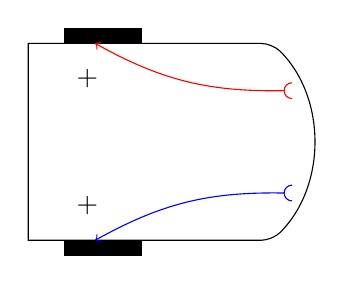
\begin{tikzpicture}[scale=.5]
% Draw big robot
\draw (-2.2cm,-2.5cm) to [rounded corners] (4cm,-2.5cm) to [rounded corners, bend right=45] (4cm,2.5cm) to (-2.2cm,2.5cm) to cycle;
\fill (-1.3cm,-2.5cm) rectangle +(2cm, -.4cm);
\fill (-1.3cm,2.5cm) rectangle +(2cm, .4cm);
\coordinate (right-wheel) at (-.5,-2.5);
\coordinate (left-wheel) at (-.5,2.5);
\node[below,xshift=-1mm,yshift=-2mm] at (left-wheel) {$+$};
\node[above,xshift=-1mm,yshift=2mm] at (right-wheel) {$+$};
% Left sensor and arrows
\coordinate (left-sensor) at (4.3,1.3);
\draw[red] (4.5, 1.5) arc[start angle=90, end angle=270, radius=.2cm];
\draw[->,red] (left-sensor) to [bend left=15] (left-wheel);
% Right sensor and arrows
\coordinate (right-sensor) at (4.3,-1.3);
\draw[blue] (4.5, -1.5) arc[start angle=270, end angle=90, radius=.2cm];
\draw[->,blue] (right-sensor) to [bend right=15] (right-wheel);
\end{tikzpicture}
\caption{Veículo covarde}\label{fig.coward}
\end{minipage}
\hspace{\fill}
\begin{minipage}{.45\textwidth}
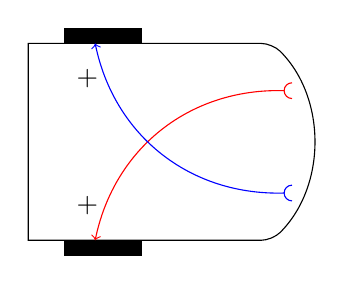
\begin{tikzpicture}[scale=.5]
% Draw big robot
\draw (-2.2cm,-2.5cm) to [rounded corners] (4cm,-2.5cm) to%
[rounded corners, bend right=45] (4cm,2.5cm) to (-2.2cm,2.5cm) to cycle;
\fill (-1.3cm,-2.5cm) rectangle +(2cm, -.4cm);
\fill (-1.3cm,2.5cm) rectangle +(2cm, .4cm);
\coordinate (right-wheel) at (-.5,-2.5);
\coordinate (left-wheel) at (-.5,2.5);
\node[below,xshift=-1mm,yshift=-2mm] at (left-wheel) {$+$};
\node[above,xshift=-1mm,yshift=2mm] at (right-wheel) {$+$};
% Left sensor and arrows
\coordinate (left-sensor) at (4.3,1.3);
\draw[red] (4.5, 1.5) arc[start angle=90, end angle=270, radius=.2cm];
\draw[->,red] (left-sensor) to [bend right=40] (right-wheel);
% Right sensor and arrows
\coordinate (right-sensor) at (4.3,-1.3);
\draw[blue] (4.5, -1.5) arc[start angle=270, end angle=90, radius=.2cm];
\draw[->,blue] (right-sensor) to [bend left=40] (left-wheel);
\end{tikzpicture}
\caption{Veículo agressivo}\label{fig.aggressive}
\end{minipage}
\end{figure}


%\begin{figure}
%\subfigures
%\begin{minipage}{\textwidth}
%\leftfigure[c]{
%\begin{tikzpicture}[scale=.5]
%% Draw big robot
%\draw (-2.2cm,-2.5cm) to [rounded corners] (4cm,-2.5cm) to [rounded corners, bend right=45] (4cm,2.5cm) to (-2.2cm,2.5cm) to cycle;
%\fill (-1.3cm,-2.5cm) rectangle +(2cm, -.4cm);
%\fill (-1.3cm,2.5cm) rectangle +(2cm, .4cm);
%\coordinate (right-wheel) at (-.5,-2.5);
%\coordinate (left-wheel) at (-.5,2.5);
%\node[below,xshift=-1mm,yshift=-2mm] at (left-wheel) {$+$};
%\node[above,xshift=-1mm,yshift=2mm] at (right-wheel) {$+$};
%% Left sensor and arrows
%\coordinate (left-sensor) at (4.3,1.3);
%\draw[red] (4.5, 1.5) arc[start angle=90, end angle=270, radius=.2cm];
%\draw[->,red] (left-sensor) to [bend left=15] (left-wheel);
%% Right sensor and arrows
%\coordinate (right-sensor) at (4.3,-1.3);
%\draw[blue] (4.5, -1.5) arc[start angle=270, end angle=90, radius=.2cm];
%\draw[->,blue] (right-sensor) to [bend right=15] (right-wheel);
%\end{tikzpicture}
%}
%\hspace{\fill}
%\rightfigure[c]{
%\begin{tikzpicture}[scale=.5]
%% Draw big robot
%\draw (-2.2cm,-2.5cm) to [rounded corners] (4cm,-2.5cm) to%
%[rounded corners, bend right=45] (4cm,2.5cm) to (-2.2cm,2.5cm) to cycle;
%\fill (-1.3cm,-2.5cm) rectangle +(2cm, -.4cm);
%\fill (-1.3cm,2.5cm) rectangle +(2cm, .4cm);
%\coordinate (right-wheel) at (-.5,-2.5);
%\coordinate (left-wheel) at (-.5,2.5);
%\node[below,xshift=-1mm,yshift=-2mm] at (left-wheel) {$+$};
%\node[above,xshift=-1mm,yshift=2mm] at (right-wheel) {$+$};
%% Left sensor and arrows
%\coordinate (left-sensor) at (4.3,1.3);
%\draw[red] (4.5, 1.5) arc[start angle=90, end angle=270, radius=.2cm];
%\draw[->,red] (left-sensor) to [bend right=40] (right-wheel);
%% Right sensor and arrows
%\coordinate (right-sensor) at (4.3,-1.3);
%\draw[blue] (4.5, -1.5) arc[start angle=270, end angle=90, radius=.2cm];
%\draw[->,blue] (right-sensor) to [bend left=40] (left-wheel);
%\end{tikzpicture}
%}
%\leftcaption{Coward vehicle\label{fig.coward}}
%\rightcaption{Aggressive vehicle\label{fig.aggressive}}
%\end{minipage}
%\end{figure}

\begin{framed}
\act{A apresentação dos veículos por Braitenberg}{brait-vehicles}
\begin{itemize}
\item Implemente os veículos de tração \emph{covarde} e de tração \emph{agressiva}.
\item Use sensores de proximidade no lugar dos sensores de luz de Braitenberg, e a detecção ou não detecção de um objeto no lugar de fontes de luz mais fortes ou mais fracas.
\item Os robôs nas Figs.~\ref{fig.loves}--\ref{fig.explorer} são os mesmos que os robôs nas Figs.~\ref{fig.coward}--\ref{fig.aggressive}, respectivamente, exceto que os valores dos sensores são negados (os sinais $-$ nas conexões): quanto mais luz for detectada, mais lenta a roda girará. Suponha que haja um valor mínimo aplicado aos motores para que as rodas girem para frente quando nenhuma fonte de luz for detectada.
\item Implemente o robô da Fig.~\ref{fig.loves}. Por que ele é chamado de \emph{amoroso}?
\item Implemente o robô na Fig.~\ref{fig.explorer}. Por que ele é chamado de \emph{explorador}?
\end{itemize}
\end{framed}

\begin{figure}
\begin{minipage}{.45\textwidth}
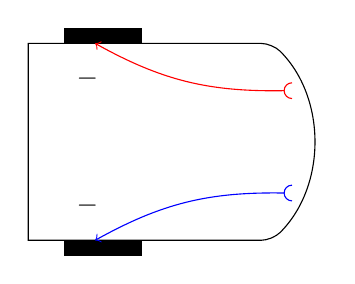
\begin{tikzpicture}[scale=.5]
% Draw big robot
\draw (-2.2cm,-2.5cm) to [rounded corners] (4cm,-2.5cm) to%
[rounded corners, bend right=45] (4cm,2.5cm) to (-2.2cm,2.5cm) to cycle;
\fill (-1.3cm,-2.5cm) rectangle +(2cm, -.4cm);
\fill (-1.3cm,2.5cm) rectangle +(2cm, .4cm);
\coordinate (right-wheel) at (-.5,-2.5);
\coordinate (left-wheel) at (-.5,2.5);
\node[below,xshift=-1mm,yshift=-2mm] at (left-wheel) {$-$};
\node[above,xshift=-1mm,yshift=2mm] at (right-wheel) {$-$};
% Left sensor and arrows
\coordinate (left-sensor) at (4.3,1.3);
\draw[red] (4.5, 1.5) arc[start angle=90, end angle=270, radius=.2cm];
\draw[->,red] (left-sensor) to [bend left=15] (left-wheel);
% Right sensor and arrows
\coordinate (right-sensor) at (4.3,-1.3);
\draw[blue] (4.5, -1.5) arc[start angle=270, end angle=90, radius=.2cm];
\draw[->,blue] (right-sensor) to [bend right=15] (right-wheel);
\end{tikzpicture}
\caption{Veículo amoroso}\label{fig.loves}
\end{minipage}
\hspace{\fill}
\begin{minipage}{.45\textwidth}
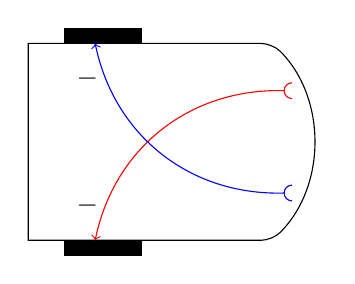
\begin{tikzpicture}[scale=.5]
% Draw big robot
\draw (-2.2cm,-2.5cm) to [rounded corners] (4cm,-2.5cm) to%
[rounded corners, bend right=45] (4cm,2.5cm) to (-2.2cm,2.5cm) to cycle;
\fill (-1.3cm,-2.5cm) rectangle +(2cm, -.4cm);
\fill (-1.3cm,2.5cm) rectangle +(2cm, .4cm);
\coordinate (right-wheel) at (-.5,-2.5);
\coordinate (left-wheel) at (-.5,2.5);
\node[below,xshift=-1mm,yshift=-2mm] at (left-wheel) {$-$};
\node[above,xshift=-1mm,yshift=2mm] at (right-wheel) {$-$};
% Left sensor and arrows
\coordinate (left-sensor) at (4.3,1.3);
\draw[red] (4.5, 1.5) arc[start angle=90, end angle=270, radius=.2cm];
\draw[->,red] (left-sensor) to [bend right=40] (right-wheel);
% Right sensor and arrows
\coordinate (right-sensor) at (4.3,-1.3);
\draw[blue] (4.5, -1.5) arc[start angle=270, end angle=90, radius=.2cm];
\draw[->,blue] (right-sensor) to [bend left=40] (left-wheel);
\end{tikzpicture}
\caption{Veículo explorador}\label{fig.explorer}
\end{minipage}
\end{figure}

%\begin{figure}
%\subfigures
%\begin{minipage}{\textwidth}
%\leftfigure[c]{
%\begin{tikzpicture}[scale=.5]
%% Draw big robot
%\draw (-2.2cm,-2.5cm) to [rounded corners] (4cm,-2.5cm) to%
%[rounded corners, bend right=45] (4cm,2.5cm) to (-2.2cm,2.5cm) to cycle;
%\fill (-1.3cm,-2.5cm) rectangle +(2cm, -.4cm);
%\fill (-1.3cm,2.5cm) rectangle +(2cm, .4cm);
%\coordinate (right-wheel) at (-.5,-2.5);
%\coordinate (left-wheel) at (-.5,2.5);
%\node[below,xshift=-1mm,yshift=-2mm] at (left-wheel) {$-$};
%\node[above,xshift=-1mm,yshift=2mm] at (right-wheel) {$-$};
%% Left sensor and arrows
%\coordinate (left-sensor) at (4.3,1.3);
%\draw[red] (4.5, 1.5) arc[start angle=90, end angle=270, radius=.2cm];
%\draw[->,red] (left-sensor) to [bend left=15] (left-wheel);
%% Right sensor and arrows
%\coordinate (right-sensor) at (4.3,-1.3);
%\draw[blue] (4.5, -1.5) arc[start angle=270, end angle=90, radius=.2cm];
%\draw[->,blue] (right-sensor) to [bend right=15] (right-wheel);
%\end{tikzpicture}
%}
%\hspace{\fill}
%\rightfigure[c]{
%\begin{tikzpicture}[scale=.5]
%% Draw big robot
%\draw (-2.2cm,-2.5cm) to [rounded corners] (4cm,-2.5cm) to%
%[rounded corners, bend right=45] (4cm,2.5cm) to (-2.2cm,2.5cm) to cycle;
%\fill (-1.3cm,-2.5cm) rectangle +(2cm, -.4cm);
%\fill (-1.3cm,2.5cm) rectangle +(2cm, .4cm);
%\coordinate (right-wheel) at (-.5,-2.5);
%\coordinate (left-wheel) at (-.5,2.5);
%\node[below,xshift=-1mm,yshift=-2mm] at (left-wheel) {$-$};
%\node[above,xshift=-1mm,yshift=2mm] at (right-wheel) {$-$};
%% Left sensor and arrows
%\coordinate (left-sensor) at (4.3,1.3);
%\draw[red] (4.5, 1.5) arc[start angle=90, end angle=270, radius=.2cm];
%\draw[->,red] (left-sensor) to [bend right=40] (right-wheel);
%% Right sensor and arrows
%\coordinate (right-sensor) at (4.3,-1.3);
%\draw[blue] (4.5, -1.5) arc[start angle=270, end angle=90, radius=.2cm];
%\draw[->,blue] (right-sensor) to [bend left=40] (left-wheel);
%\end{tikzpicture}
%}
%\leftcaption{Loves vehicle\label{fig.loves}}
%\rightcaption{Explorer vehicle\label{fig.explorer}}
%\end{minipage}
%\end{figure}

\section{Sumário}

Um robô exibe comportamento reativo quando suas ações dependem apenas dos valores atuais retornados por seus sensores. Este capítulo apresentou duas famílias de comportamento reativo. Os veículos Braitenberg implementam o comportamento reativo alterando a configuração dos motores em resposta aos eventos dos sensores de proximidade que detectam ou não um objeto em alguma posição em relação ao robô. Os veículos demonstram que um comportamento complexo pode resultar de algoritmos relativamente simples.

O seguimento de linha é uma tarefa fundamental na robótica. Devido às incertezas do movimento do robô e seu ambiente, os robôs usam pontos de referência como linhas para garantir que eles se movam ao seu destino pretendido. O seguimento de linha é um comportamento reativo porque o robô modifica seu comportamento em resposta aos valores retornados pelos sensores de solo. Demos três configurações para o robô e para a linha, e desenvolvemos algoritmos para cada caso. O desempenho dos algoritmos depende dos limites dos sensores e das velocidades dos motores, que devem ser determinados por experimentos para garantir que o robô se mova rapidamente enquanto se mantém robusto às mudanças no ambiente.

\section{Leitura adicional}

O livro de Braitenberg \cite{valentino} é interessante porque ele escreve a partir da perspectiva de um neurocientista. O livro descreve veículos que utilizam tecnologia imaginada, mas que, no entanto, são instigantes ao pensamento. Os veículos Braitenberg aqui descritos são adaptados das implementações de hardware descritas em \cite{creatures}. Uma implementação dos veículos Braitenberg em Scratch pelo primeiro autor pode ser encontrada em:\par\noindent\url{https://scratch.mit.edu/studios/1452106}.

